\cleardoublepage
\chapter{外文翻译}

\sectionnonum{K-EmoCon:用于自然对话中连续情感识别的多模式传感器数据集}
\textbf{摘要:}随着低成本移动传感器的普及,情感识别在社交互动中的潜在应用前景逐渐显现出来,但同时也面临着缺乏自然情感互动数
据的挑战。大多数现有的情绪数据集是在有限环境中收集的,并不支持研究在自然状态下产生的特殊情绪。
因此,研究社会互动背景下的情绪需要一个全新的数据集,而K-EmoCon就是这样一个对自然对话中连续情绪
进行全面注释的多模态数据集。它运用现成设备,在16场(每场约10分钟)有关社会问题的配对辩论中进行多模态测量
,测量值包括视听记录、脑电图和外周生理信号等。与之前数据集不同的是,它采用了来自三个可用视角的情感注释:
自我、辩论同伴和外部观察员。评审员在观看辩论录像时,每隔5秒对情绪表现(包括唤起效价和18种额外的分类情绪)
进行注释,由此产生的K-EmoCon是适用于社会互动中情绪多视角评估的第一个公开可用的情绪数据集。

% \textbf{关键词:} 1 2 3
\section{背景和总结}
情绪识别研究旨在赋予计算机识别情绪的能力,它是创造能够理解甚至表达情感的机器的基础,
而这一套识别、理解和表达情绪的技能构成了我们所谓的情商。研究表明,情商对于个体在社会中的导向是非常必要的
,因为它能够引导一个人判断事物是否可取,并相应地规范自己和他人的行为。

那么为什么机器需要情感技能?随着机器学习和人工智能的进步,在社会的各个领域,
包括那些需要专业知识的领域,如医疗预后/诊断或汽车驾驶,从人类到机器的过渡已经显而易见。细分领域的人工智能系统似乎不可避免地在各自的领域超越了人类专家,这一点已经被AlphaGo在围棋比赛中超越人类棋王的出色表现所证明。

\raggedbottom
不过,尽管人工智能拥有超人的能力,但并非所有的人工智能都会与人类竞争。相反,许多人工智能系统会与我们合作或为我们服务,
而情商在这种人机交互系统中发挥了至关重要的作用。想象一下,当用户回家时,一个智能音箱会愉快地打招呼。
但当用户度过了不愉快的一天时,音箱又该如何问候?忽视用户情绪状态的音箱可能会加重用户的负担,
但意识到用户心情的智能音箱可以保持沉默以避免麻烦。同样,对于设计用于复杂任务的人工智能系统来说,情商也至关重要。
例如,在自动驾驶和人工驾驶混合的道路上,准确识别人类驾驶员的情绪能够使自动驾驶汽车更好地判断人类驾驶员的意图,
从而带来更高的安全性。

现在,机器要想拥有情商,就必须首先学会识别情绪,而学习的先决条件就是数据。然而,在情绪数据的获取方面还存在一些挑战。
虽然情绪是普遍存在的,但要准确地衡量它们是困难的。情绪通常被认为是通过面部表情表达的心理状态,它有不同的类别。
但后续研究却产生了完全相反的结论,面部表情不是清晰的,而是复合的、相对的和具有误导性的。
最近一篇对相关科学证据的综述也反对这一普遍观点,认为面部表情缺乏可靠性、专一性和概括性,
过去对情境依赖性和情绪的个体可变性的研究也是如此。

情绪这种内在的隐蔽性使得现有的许多情绪数据集不适合在自然状态下研究情绪。
大多数情绪数据集由静态环境(即实验室)中挑选的特定刺激所诱发的情绪组成。
这种方法使得实验者能够完全控制数据的收集,并进一步对特定的情感行为进行评估以及通过先进技术(如神经影像学)
获取精密细粒度的数据。然而,实验室生成的数据对现实场景的概括性很差,因为它们经常包含典型情绪的强烈表达,
而这在现实世界中是很少能被观察到的,并且只是从一小部分人群中所获得。

另一种利用媒体内容和众包的方法,弥补了传统方法的缺陷。丰富的网络内容,如电视节目和电影,
使得研究人员能够有效收集各种背景下的丰富情感数据;众包则在作为另一个数据源的同时,
进一步支持完成成本较低的数据注释。这种类型的数据集在样本量和受试者多样性方面具备优势,
但存在普遍性方面的缺陷。基于媒体内容的数据集,其情感展示通常由专业演员通过假想情境而产生,
而这种情感描绘与自发的情感表达是否相似以及有多大程度相似仍然存在争议。同时,这类数据集也无法获取生理信号,
而生理信号恰恰被认为是检测微弱情绪状态变化的关键信息。

为了弥补在识别自然情绪方面数据集的缺陷,我们引入了K-EmoCon,这是一个从32名被试(两两成组进行有关社会问题的辩论)
中采集的多模式数据集。它包括用三个现成可穿戴设备收集的生理传感器数据、辩论期间参与者的视听录像以及连续情绪注释。
据我们所知,K-EmoCon也是第一个从所有可能角度(被试主体、辩论伙伴和外部观察者)进行情感注释的数据集。

\section{方法}
\subsection{数据集的设计}
\subsubsection{预期的用途}
受之前研究对话中情绪变化的工作启发,K-EmoCon的设计考虑到了一个包含能够不受干扰地跟踪生理信号的可穿戴设备在内的双人社会互动场景。该数据集旨在对情绪进行多视角分析,具体目标如下:
\begin{enumerate}
    \item 拓展对情绪表达的多视角研究,提高其自动识别能力。
    \item 为研究如何以多角度多方式,尤其是在社会互动背景下感知情感提供一个新的机会。
    \end{enumerate}

之前的研究表明,从多个来源进行情绪注释可以提高其识别的准确性。然而目前,还没有任何研究在情绪注释中使用这三个可用视角(即被试者本人、互动同伴和外部观察者)。进行多视角研究关系到在情感注释中建立基础真理的问题。情绪本质上是一种内在现象,其机制无法被外部所审查,即使是体验情绪的个体本身也无法考究。因此,情绪可能不存在基础真理。我们应该把外部观察者对于情绪最认同的东西作为基本真理,还是把经历情绪的个体所反馈的感受作为基本真理?如果情绪是强烈和纯粹的,那么两种观点可能是一致的,但如前所述,这样的情绪是罕见的。所以相反,自我报告和观察到的情绪可能会因为各种原因而不一致。可能是因为人们常常隐藏自己的真实情感,可能是因为人们有时并没有完全注意到自己的内心状态,也可能是因为有些人在理解或表达情感上有困难。

借助K-EmoCon,我们希望能够在涉及三个方面的社会互动背景下,将三个可用视角纳入情绪注释,对这些情绪与认知不匹配的案例进行一个比较全面地研究:
\begin{enumerate}
    \item 主体——是直接体验情绪并产生自我注解的人,尤其是“感觉”情绪的来源。
    \item 同伴——是与主体互动的人,间接体验主体的情感;因此,他/她对引发被试情绪的互动能够进行情境回顾,并在此基础上做出同伴注释。
    \item 外部观察者——是那些观察实验对象情绪的人,他们不能够对诱发情绪的互动进行确切情境的回顾,所以产生的是外部观察者注释。
    \end{enumerate}

请注意,虽然我们对情绪注释的视角的定义与其他研究人员之前使用的定义相似(自我报告与感知/观察),但我们还根据观察者是否拥有实验主体产生情绪时的情境信息对观察者注释的类别进行了进一步的分割,因为我们希望考虑情境信息在情绪感知和识别中的作用。

在这个问题上,现有的对话情绪数据集范围十分有限,因为它们最多包含来自主体和外部观察者两个视角的情绪注释,
而忽略了来自参与对话的其他人(我们称之为同伴)的注释。或者在特定研究目标下,部分数据集只考虑一种特定类型的注释
又或者它们的设计不允许获取多视角的注释(例如,一个基于电视节目对话构建的数据集,只允许收集外部观察者的注释)。
K-EmoCon与现有情感数据集的区别见\autoref{tab:Comparison}。

% Please add the following required packages to your document preamble:
%\usepackage[table,xcdraw]{xcolor}
% If you use beamer only pass "xcolor=table" option, i.e. \documentclass[xcolor=table]{beamer}
\begin{table}[htbp]
    \centering
    \footnotesize
    \setlength{\abovecaptionskip}{-0.1cm}
    \setlength{\belowcaptionskip}{0.2cm}
    \renewcommand\arraystretch{1.5}
    \caption[K-EmoCon数据集与现有多模态情感识别数据集的比较。]{K-EmoCon数据集与现有多模态情感识别数据集的比较。Posed.是指被试按照指示去表现一种
    \protect\\[4.5pt]特定的情绪;Spon.即自发产生的情绪。Induced.是指用选定刺激物去诱发情绪。注释类型中,S为自
    \protect\\[4.5pt]我注释,P为同伴注释,E为外部观察者注释。1)如果在数据收集中涉及到脚本化的互动,即使没有使
    \protect\\[4.5pt]用人工刺激物(如情感诱导的视频片段),该数据集也被认为包含诱发的情感。2)实验采用预先定义的
    \protect\\[4.5pt]刺激情绪类别和参与者在认知任务中的成功率作为基础真实标签。}
    \label{tab:Comparison}
    \begin{tabular}{|l|l|l|l|l|l|l|l|}
    \hline
    %\rowcolor[HTML]{F6AE72} 
    {\color[HTML]{333333} \textbf{名称(年份)}}                      & \textbf{容量} & \textbf{实验范式}                                                                                   & \textbf{\begin{tabular}[c]{@{}l@{}}自发/\\ 引导\end{tabular}} & \textbf{\begin{tabular}[c]{@{}l@{}}自然/\\ 诱发\end{tabular}} & \textbf{注释方法}                                      & \textbf{注释类型} & \textbf{实验环境}                                      \\ \hline
    \begin{tabular}[c]{@{}l@{}}IEMOCAP\\ (2008)\end{tabular}    & 10          & \begin{tabular}[c]{@{}l@{}}视频、面部动作捕捉、\\ 手势、语音(音频和转录)\end{tabular}                               & \begin{tabular}[c]{@{}l@{}}两者\\ 都有\end{tabular}                                                   & \begin{tabular}[c]{@{}l@{}}两者\\ 都有\end{tabular}                                                       & 每次对话                                               & S,E           & 互动形式                                               \\ \hline
    \begin{tabular}[c]{@{}l@{}}SEMAINE\\ (2011)\end{tabular}    & 150         & \begin{tabular}[c]{@{}l@{}}视频,FAUs,演讲\\ (音频和转录)\end{tabular}                                    & 自发                                                          & 诱发                                                        & 连续跟踪                                               & E             & 互动形式                                               \\ \hline
    \begin{tabular}[c]{@{}l@{}}MAHNOB-HCI\\ (2011)\end{tabular} & 27          & \begin{tabular}[c]{@{}l@{}}视频(面部和身体)、\\ 眼睛注视、音频、生物信号\\ (EEG、GSR、ECG、呼吸、\\ 皮肤温度)\end{tabular}    & 自发                                                          & 诱发                                                        & 每个刺激                                               & S             & 个人                                                 \\ \hline
    \begin{tabular}[c]{@{}l@{}}DEAP\\ (2012)\end{tabular}       & 32          & \begin{tabular}[c]{@{}l@{}}脸部视频,生物信号\\ (EEG、GSR、BVP、呼吸、\\ 皮肤温度、EMG和EOG)\end{tabular}            & 自发                                                          & 诱发                                                        & 每个刺激                                               & S             & 个人                                                 \\ \hline
    \begin{tabular}[c]{@{}l@{}}DECAF\\ (2015)\end{tabular}      & 30          & \begin{tabular}[c]{@{}l@{}}近红外人脸视频,生物信号\\ (EEG、hEOG、ECG、TEMG)\end{tabular}                      & 自发                                                          & 诱发                                                        & 每个刺激                                               & S             & 个人                                                 \\ \hline
    \begin{tabular}[c]{@{}l@{}}ASCERTAIN\\ (2016)\end{tabular}  & 58          & \begin{tabular}[c]{@{}l@{}}面部运动单元(EMO),\\ 生物信号(ECG、GSR、EEG)\end{tabular}                        & 自发                                                          & 诱发                                                        & 每个刺激                                               & S             & 个人                                                 \\ \hline
    \begin{tabular}[c]{@{}l@{}}MSPIMPROV\\ (2016)\end{tabular}  & 12          & 面部视频,语音音频                                                                                       & \begin{tabular}[c]{@{}l@{}}两者\\ 都有\end{tabular}                                                        & \begin{tabular}[c]{@{}l@{}}两者\\ 都有\end{tabular}                                                       & 每次对话                                               & E             & 互动形式                                               \\ \hline
    \begin{tabular}[c]{@{}l@{}}DREAMER\\ (2017)\end{tabular}    & 23          & 生物信号(EEG、ECG)                                                                                   & 自发                                                          & 诱发                                                        & 每个刺激                                               & S             & 个人                                                 \\ \hline
    \begin{tabular}[c]{@{}l@{}}AMIGOS\\ (2018)\end{tabular}     & 40          & \begin{tabular}[c]{@{}l@{}}录像(面部和身体),\\ 生物信号(EEG、ECG、GSR)\end{tabular}                          & 自发                                                          & 诱发                                                        & 每个刺激                                               & S,E           & \begin{tabular}[c]{@{}l@{}}个人、\\ 团体\end{tabular}   \\ \hline
    \begin{tabular}[c]{@{}l@{}}MELD\\ (2019)\end{tabular}       & 7           & 视频,演讲(音频和转录)                                                                                    & \begin{tabular}[c]{@{}l@{}}两者\\ 都有\end{tabular}                                                        & \begin{tabular}[c]{@{}l@{}}两者\\ 都有\end{tabular}                                                       & 回合制                                                & E             & \begin{tabular}[c]{@{}l@{}}同伴式,\\ 小组式\end{tabular} \\ \hline
    \begin{tabular}[c]{@{}l@{}}CASE\\ (2019)\end{tabular}       & 30          & \begin{tabular}[c]{@{}l@{}}生物信号(ECG、呼吸、\\ BVP、GSR、皮肤温度、EMG)\end{tabular}                        & 自发                                                          & 诱发                                                        & 连续跟踪                                               & S             & 个人                                                 \\ \hline
    \begin{tabular}[c]{@{}l@{}}CLAS\\ (2020)\end{tabular}       & 64          & \begin{tabular}[c]{@{}l@{}}生物信号(ECG、PPG、EDA),\\ 加速器\end{tabular}                                & 自发                                                          & 诱发                                                        & \begin{tabular}[c]{@{}l@{}}每个刺激/\\ 任务\end{tabular} & 预定义           & 个人                                                 \\ \hline
    \textit{\begin{tabular}[c]{@{}l@{}}K-EmoCon\\ (2020)\end{tabular}}   & 32          & \begin{tabular}[c]{@{}l@{}}视频(面部、手势)、\\ 语音音频、加速度计、\\ 生物信号(EEG、ECG、BVP、\\ EDA、皮肤温度)\end{tabular} & 自发                                                          & 自然                                                        & 连续区间                                               & S,P,E         & 互动形式                                               \\ \hline
    \end{tabular}
    \end{table}

\subsubsection{数据收集的背景}
在这个方面,我们设置了一个同伴随机分配的半结构化轮流辩论(主题为社会问题相关),作为数据收集的环境。这种设置适合收集日常生活中可能自然产生的情绪,因为它与个体可能在工作场所进行的社会互动相类似。

同时,这种设置也特别适合研究对情绪的错误认知,因为同伴是随机分配的,足够正式和自发。我们期望通过环境的这种正式性和自发性,迫使参与者以一种适当的社会方式调节自己的情绪,进而让我们能观察到参与者不太明显并且更可能被同伴所误解的情绪。

\subsubsection{数据收集装置}
我们选择移动、可穿戴和低成本的设备来收集情感生理信号和视听记录,主要目的是希望基于我们实验数据的发现能够更具可重复性和可扩展性,同时也是考虑到我们实验目标的具体实施,即在自然状态下调查情感与感知的不匹配。研究表明,融合隐形和显性的情感信息,可以使我们更准确地识别专业演员微妙的情感表达。然而,据我们所知,没有一项研究在未经过专业表演训练并处于自然社会互动情境下的群体中实现类似的结果。因此,我们的数据集是一个进一步的探索,以检验在沟通过程中,非专业演员群体产生的较低强度情绪是否可以被准确识别。

如果微弱情绪的准确检测是可能实现的,那么能否进一步利用它们标志出在沟通过程中被误解的情绪将会是一次有趣的探索。同样,在存在大量背景信息的社交互动中,情感强度在多大程度上影响解码的准确性,也非常值得探索。K-EmoCon可以对这些问题进行深入地研究。

此外,我们还考虑到促进情感交流的移动可穿戴技术的使用情况。研究人员正在积极探索如何利用可穿戴设备在与他人交流情感和心理状态时收集富有表现力的生物信号。我们的数据集可以为基于生物信号的相关辅助技术研究做出贡献,通过分析恰当的情绪交流时刻来实现合适的情感交流。
\subsection{伦理申明}
K-EmoCon数据集的构建得到了韩国科学技术院(KAIST)机构审查委员会的批准。委员会还审查并批准了同意书,具体包括数据收集目的、数据收集程序、从参与者中收集得到的数据类型、为参与者提供的补偿,以及保护隐私敏感数据的协议等。

参与者到达数据收集地点后,充分阅读同意书(内容相同)并签署书面同意,表示愿意参与此项数据收集工作。由于K-EmoCon将向公众开放,因此在公开包含个人身份信息(PII)的数据(辩论期间参与者的视听片段,包括他们的脸和声音)时,需要获得每个参与者的同意。参与者同时也被告知,实验的参与遵循自愿原则,他们可以在任何时候终止数据的收集。最后公开的K-EmoCon数据集包括32名参与者中同意公开其个人信息的21名参与者的视听记录,不含剩余不同意公开的11名参与者的相关数据。
\subsection{参与者招募和准备}
我们在2019年1月至3月间招募了32名被试。首先,我们在KAIST学生社区的在线公告板上发布了一则有关 "辩论中的情绪感应 "的实验招募公告。实验具体要求参与者就韩国济州岛接受也门难民的问题进行10分钟的辩论;同时还要求辩论必须用英语进行,即参与者应该能够流利地使用英语发言,但不一定要达到母语水平。具体来说,参与者至少需要有三年在以英语为母语的国家生活的经验,或在以下任意一项标准化英语口语测试中达到相应标准:TOEIC口语7级、TOEFL口语27分或IELTS口语7级。

确定每个被试参与数据收集的日期和时间后,我们会通过电子邮件发送四篇关于济州岛也门难民危机主题的新闻文章,包括两篇中立观点的文章,一篇支持难民和另一篇反对难民的文章。参与者应按照要求事先阅读这些文章,以熟悉辩论主题。

所有被试都是KAIST的学生,年龄从19岁到36岁不等(平均年龄23.8岁,标准差3.3岁),性别和国籍各不相同。
我们根据参与者反馈的时间安排,将他们随机配对成16组。参试者的性别、国籍和年龄的分类见\autoref{tab:Debates}。
\begin{table}[htbp]
    \centering
    \footnotesize
    \setlength{\abovecaptionskip}{-0.1cm}
    \setlength{\belowcaptionskip}{0.2cm}
    \renewcommand\arraystretch{1.5}
    \caption[辩论组别及参与者信息。]{辩论组别及参与者信息。}
    \label{tab:Debates}
    \begin{tabular}{|lp{2cm}|lp{2cm}|}
    \hline
    \multicolumn{2}{|l|}{参与者}       & \multicolumn{2}{l|}{性别和年龄}         \\ \hline
    \multicolumn{1}{|p{2cm}|}{P1}  & P2  & \multicolumn{1}{p{2cm}|}{M(25)} & M(23) \\ \hline
    \multicolumn{1}{|p{2cm}|}{P3}  & P4  & \multicolumn{1}{p{2cm}|}{M(36)} & M(25) \\ \hline
    \multicolumn{1}{|l|}{P5}  & P6  & \multicolumn{1}{l|}{M(22)} & M(23) \\ \hline
    \multicolumn{1}{|l|}{P7}  & P8  & \multicolumn{1}{l|}{M(22)} & F(22) \\ \hline
    \multicolumn{1}{|l|}{P9}  & P10 & \multicolumn{1}{l|}{M(21)} & M(22) \\ \hline
    \multicolumn{1}{|l|}{P11} & P12 & \multicolumn{1}{l|}{M(22)} & M(25) \\ \hline
    \multicolumn{1}{|l|}{P13} & P14 & \multicolumn{1}{l|}{M(22)} & F(21) \\ \hline
    \multicolumn{1}{|l|}{P15} & P16 & \multicolumn{1}{l|}{M(30)} & F(26) \\ \hline
    \multicolumn{1}{|l|}{P17} & P18 & \multicolumn{1}{l|}{M(21)} & M(20) \\ \hline
    \multicolumn{1}{|l|}{P19} & P20 & \multicolumn{1}{l|}{M(21)} & F(23) \\ \hline
    \multicolumn{1}{|l|}{P21} & P22 & \multicolumn{1}{l|}{M(25)} & F(25) \\ \hline
    \multicolumn{1}{|l|}{P23} & P24 & \multicolumn{1}{l|}{M(22)} & F(29) \\ \hline
    \multicolumn{1}{|l|}{P25} & P26 & \multicolumn{1}{l|}{F(26)} & M(25) \\ \hline
    \multicolumn{1}{|l|}{P27} & P28 & \multicolumn{1}{l|}{F(24)} & F(23) \\ \hline
    \multicolumn{1}{|l|}{P29} & P30 & \multicolumn{1}{l|}{F(23)} & F(24) \\ \hline
    \multicolumn{1}{|l|}{P31} & P32 & \multicolumn{1}{l|}{M(24)} & F(19) \\ \hline
    \end{tabular}
    \end{table}
\subsection{数据收集设置}
所有的数据收集环节都是在两个温度和光照可控的房间内进行的。两名参与者面对面坐在一张桌子上,
中间相隔一定距离以保证交流的舒适程度(见\autoref{fig:Debates})。两部三星Galaxy S7智能手机通过三脚架固定在桌子中间,
分别面向一位参与者,从第二人称视角(POV)捕捉其面部表情和上半身的运动,同时通过相机应用捕捉语音。

在辩论中,参与者佩戴了一套可穿戴的传感器,如\autoref{fig:Equipment}所示,其中包括:
\begin{enumerate}
\item Empatica E4腕带 —— 采集了光电容积描记(PPG)、三轴加速度、体温和皮肤电活动(EDA)。心率和心跳间期(IBI)由PPG传感器测量的血容量脉冲(BVP)计算得出。
\item Polar H7蓝牙心率传感器 —— 使用心电图(ECG)传感器检测心率,用于补充E4中的PPG传感器,该传感器容易受运动影响。
\item NeuroSky MindWave耳机 —— 通过两个干式传感器电极收集脑电图(EEG)信号,一个在前额(额叶的fp1通道-10/20系统),一个在左耳垂(参考电极)。
\item LookNTell头戴式摄像机 —— 在塑料圆环一端连接摄像机,佩戴在参与者头部,以第一人称POV的方式拍摄视频。
\end{enumerate}

% 所有列出的设备都可以在移动环境下运行。Empatica E4将数据保存在设备上,并上传到电脑上。
% Polar H7传感器和MindWave耳机可以通过低功耗蓝牙(BLE)与移动电话通信存储数据。
% 每个设备收集数据的采样率和信号范围\autoref{tab:Collected-Data}。

\begin{figure}[htbp]
    \centering
    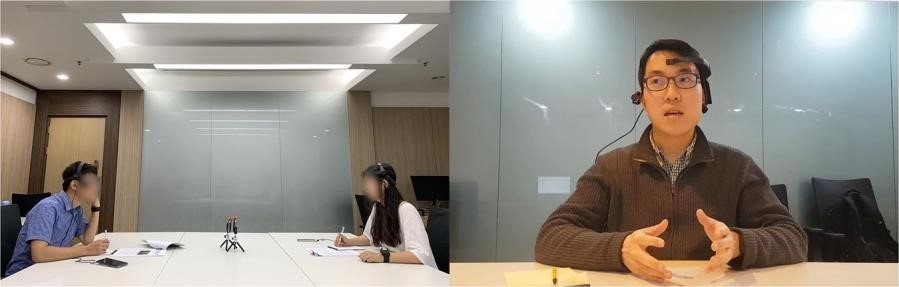
\includegraphics[width=.75\linewidth]{debate.jpg}
    \caption[辩论图片]{左图显示一组参与者坐在桌前准备辩论。桌子中间三脚架上的两部智能手机(红色标注)记录了参与者的面部表情和上半身动作(如右图所示)}{\label{fig:Debates}}
\end{figure}
\begin{figure}[htbp]
    \centering
    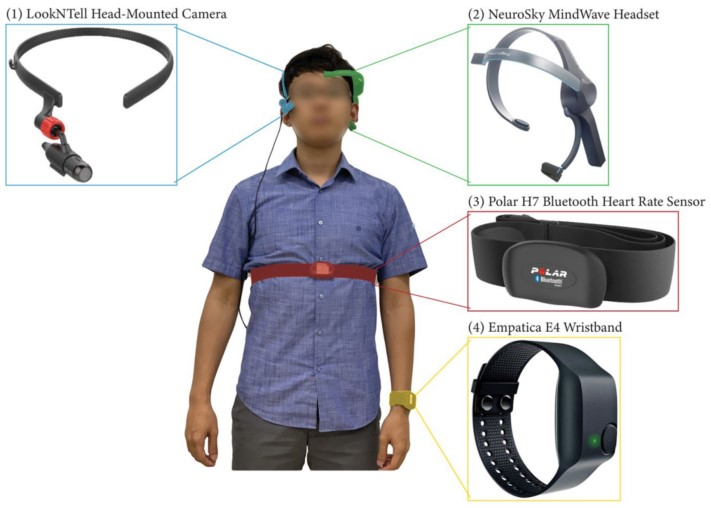
\includegraphics[width=.75\linewidth]{equipment.jpg}
    \caption[设备图片]{配备可穿戴传感器的参与者的正面视图。}{\label{fig:Equipment}}
\end{figure}

所有列出的设备都可以在移动环境下运行。Empatica E4将数据保存在设备中,并随后上传至电脑上。
Polar H7传感器和MindWave耳机可以通过低功耗蓝牙(BLE)与移动电话通信,并存储数据。
每个设备收集的数据的及其采样率和信号范围见\autoref{tab:Collected-Data}。

% Please add the following required packages to your document preamble:
% \usepackage{multirow}
% \begin{table}[htbp]
%     \centering
%     \footnotesize
%     \setlength{\abovecaptionskip}{-0.1cm}
%     \setlength{\belowcaptionskip}{0.2cm}
%     \renewcommand\arraystretch{1.5}
%     \caption[每个可穿戴设备收集的数据及其采样率和信号范围。]{每个可穿戴设备收集的数据及其采样率和信号范围。}
%     \label{tab:Collected-Data}
%     \begin{tabular}{|l|l|p{2cm}|l|}
%     \hline
%     设备                                   & 收集的数据         & 采样率   & 信号范围[最小,最大]    \\ \hline
%     \multirow{6}{*}{Empatica E4腕带}       & 3轴加速器         & 32Hz  & [-2g,2g]       \\ \cline{2-4} 
%                                          & BVP (PPG)     & 64Hz  & 不适用            \\ \cline{2-4} 
%                                          & EDA           & 4Hz   & [0.01μS,100μS] \\ \cline{2-4} 
%                                          & 心率(来自BVP)     & 1Hz   & 不适用            \\ \cline{2-4} 
%                                          & IBI (来自BVP)   & 不适用   & 不适用            \\ \cline{2-4} 
%                                          & 体温            & 4Hz   & [-40°C,115°C]  \\ \hline
%     \multirow{2}{*}{NeuroSky MindWave耳机} & 脑电波(fp1通道脑电图) & 125Hz & 不适用            \\ \cline{2-4} 
%                                          & 注意力与冥想        & 1Hz   & [0, 100]       \\ \hline
%     Polar H7心率传感器                        & 心率(心电图)       & 1Hz   & 不适用            \\ \hline
%     \end{tabular}
%     \end{table}
\subsection{数据收集程序}
\subsubsection{管理}
所有的数据收集流程分四个阶段进行:(1)实验引导,(2)基线测量,(3)辩论和(4)情绪注释。
每个环节都各有两名实验人员进行管理(数据收集程序的概述见\autoref{tab:Collected-Steps}),其中一名实验人员在辩论期间担任主持人,
提醒参与者辩论的剩余时间,并在必要情况下进行干预(如辩论过于激烈,或参与者超出2分钟的规定辩论时长)。
\begin{table}[htbp]
    \centering
    \footnotesize
    \setlength{\abovecaptionskip}{-0.1cm}
    \setlength{\belowcaptionskip}{0.2cm}
    \renewcommand\arraystretch{1.5}
    \caption[每个可穿戴设备收集的数据及其采样率和信号范围。]{每个可穿戴设备收集的数据及其采样率和信号范围。}
    \label{tab:Collected-Data}
    \begin{tabular}{|l|l|p{2cm}|l|}
    \hline
    设备                                   & 收集的数据         & 采样率   & 信号范围[最小,最大]    \\ \hline
    \multirow{6}{*}{Empatica E4腕带}       & 3轴加速器         & 32Hz  & [-2g,2g]       \\ \cline{2-4} 
                                         & BVP (PPG)     & 64Hz  & 不适用            \\ \cline{2-4} 
                                         & EDA           & 4Hz   & [0.01μS,100μS] \\ \cline{2-4} 
                                         & 心率(来自BVP)     & 1Hz   & 不适用            \\ \cline{2-4} 
                                         & IBI (来自BVP)   & 不适用   & 不适用            \\ \cline{2-4} 
                                         & 体温            & 4Hz   & [-40°C,115°C]  \\ \hline
    \multirow{2}{*}{NeuroSky MindWave耳机} & 脑电波(fp1通道脑电图) & 125Hz & 不适用            \\ \cline{2-4} 
                                         & 注意力与冥想        & 1Hz   & [0, 100]       \\ \hline
    Polar H7心率传感器                        & 心率(心电图)       & 1Hz   & 不适用            \\ \hline
    \end{tabular}
    \end{table}
\begin{table}[htbp]
    \centering
    \footnotesize
    \setlength{\abovecaptionskip}{-0.1cm}
    \setlength{\belowcaptionskip}{0.2cm}
    \renewcommand\arraystretch{1.5}
    \caption[数据收集的流程。]{数据收集的流程。每个完整流程大约持续两个小时。}
    \label{tab:Collected-Steps}
    \begin{tabular}{|p{3cm}|p{2cm}|l|}
    \hline
    实验步骤      & 限制时长 & 描述                                                                                 \\ \hline
    阅读并签署同意书  &10分钟 & \begin{tabular}[c]{@{}l@{}}实验者向参与者提供同意书,\\ 并收集参与和收集隐私敏感数据的两份书面同意书。\end{tabular}    \\ \hline
    选择辩论双方和顺序 &5分钟  & 参与者被分配到支持或反对接受难民的论点,并决定发言次序。                                                       \\ \hline
    准备辩论      &15分钟 & 参与者获得补充材料,并准备论点。                                                                   \\ \hline
    穿戴传感器     &10分钟 & 实验者向参与者解释可穿戴设备并协助穿戴。                                                               \\ \hline
    基线测量      &2分钟  & 测量每位参与者的基线状态(对应中性状态)。                                                              \\ \hline
    辩论简介      &5分钟  & 主持人解释辩论规则,允许参与者随时提问。                                                               \\ \hline
    正式辩论      &10分钟 & \begin{tabular}[c]{@{}l@{}}参与者在轮流发言时可连续发言两分钟\\ (辩论结束前30秒和60秒会分别得到提示)。\end{tabular} \\ \hline
    情绪注释      &60分钟 & \begin{tabular}[c]{@{}l@{}}参与者观看自己和同伴的录像,\\ 并进行情绪注释(5秒为一时间间隔)。\end{tabular}        \\ \hline
    \end{tabular}
    \end{table}
\subsubsection{实验引导}
每位参与者在实验前都会得到一份同意书。同意书向参与者申请两个书面同意,第一是同意参与数据收集,这是强制性的;第二是同意配合公开在实验期间收集的个人隐私敏感数据,这一项参与者可以拒绝。

参与者同意参与研究后,需阐述自己关于接纳济州岛也门难民的观点(支持或反对)。参与者可以通过简短的讨论来确定自己偏好的立场,或通过抛硬币随机决定。后续决定辩论中发言次序的流程也与此相同。

接下来,参与者有15分钟的时间来准备他们的论点。每位参与者获得的材料包括笔和纸,以及他们之前通过电子邮件收到的文章打印件。在他们准备完毕后,实验人员需要为参与者配备可穿戴设备。E4腕带佩戴在参与者的非惯用手,以减少手臂运动对PPG测量准确度的影响。实验人员必须保证腕带紧固以及电极与参与者皮肤接触良好,同时还需保证脑电图耳机和头戴式摄像机与参与者头部完全吻合,必要时手动调整头戴式摄像机的镜头,以确保捕捉到的视图与参与者的主观视图相近。连接Polar H7传感器的柔性带绑在参与者胸部,使电极和皮肤良好接触,最后将传感器放置在参与者太阳穴上方。

\subsubsection{基线测量}
所有设备佩戴完成后,我们会先要求参与者观看一个短片,并通过传感器测量其基线数据,构成每个参与者的中性状态。这一步在构建情绪数据集中非常常用,特别是在重复测量时,能够很明显地减少个人偏见和以前情绪状态的影响。

各个研究团队用于基线测量的流程通常会根据实验目的而做调整。在基于刺激的实验中,研究人员在被试观看能够诱发中性情绪状态的刺激时进行测量,如果是连续多次测量,则在刺激之间测量静止状态活动。在K-EmoCon的实验中,参与者观看的是Color Bars片段(经Gross团队评估,为能够诱发中性情绪的视频材料)。实验人员必须确保在基线测量期间没有设备故障的情况。

\subsubsection{辩论}
主持人示意后,辩论开始,持续约10分钟。整个辩论过程中,参与者的面部表情、上半身动作和发言都会被记录。组内两位参与者轮流发言,单次发言时长限制两分钟。同时,参与者允许在对手的轮次中发言,以保证更加自然的交流氛围。主持人在每位参与者发言结束前30秒和60秒进行提示,若超过时长限制则进行干预。辩论在10分钟时结束,但如果最后一位发言者还未完成其论点,允许一定的时长灵活性。

\subsubsection{情绪注释}
完成辩论后,参与者需要休息15分钟,然后在电脑上对自己和同伴在辩论中的情绪进行注释。具体来说,每个参与者观看他/她自己的一段视听录像以及同伴的另一段记录(都为第二人称POV记录,包括面部表情、上身动作和发言),从辩论开始到结束,每隔5秒注释一次情绪。5秒这一时间间隔的选择主要是依据Busso等人的研究(即在IEMOCAP中发言人情绪转变的平均时间约为4.5秒)以及语言学研究的相关结果。

我们采用的注释方法,是一种回溯性的情感判断方法,它在情感计算中被广泛用于收集情感的自我报告,特别是在被试需要不间断参与的情感诱导过程中。我们选择这种方法,主要是希望能够使参与者更加自然地互动,进而提升最终获得情绪数据的质量。

需要注意的是,我们没有向参与者提供从头戴式摄像机拍摄的第一人称POV录像,他们只能通过第二人称POV录像来注释感受到的情绪。在这个选择上可能存在一个疑虑,即参与者观看自己的面部录像会不会将其视角转变成一个类似于观察者的视角,从而导致他们对当时情绪感受不自然、不准确。然而事实上,摄像头录像可能反而是一个更加自然的工具,因为参与者可以更加直观地从具身角度来回忆他们在过去特定时刻的感觉。

同时,我们发现头戴式摄像头所捕捉到的信息范围不足以准确注释感受到的情绪。实验人员手动调整了头戴式摄像头的镜头,使得录像与参与者的主观视角相似,但头戴式摄像头的录像缺少相对细微的信息,如参与者的眼神。此外,有研究表明,情绪记忆很容易出现偏差和失真。所以在这一方面,与正面面部录像相比,头戴式摄像机拍摄的第一人称POV录像所包含的信息十分有限,并且很容易导致对情绪的错误注释,尤其是在回忆的过程中。我们进一步注意到,其实个体从面部推测情绪的情况并不少见,比如在日常生活中照镜子或自拍等等。

因此,参与者最终观看和注释的是他们的第二人称录像。参与者总共标注出了20个不同类别的情绪,如\autoref{tab:Collected-Annotation}所示。
实验人员在整个注释过程中为参与者提供帮助:开始注释之前,实验人员需要向参与者解释各个情绪类别,
帮助他们正确理解每个项目的含义和具体的注释流程。同时,实验人员还需明确告知参与者,是标注当时个人感受到的情绪,
而不是当下通过面部表情等感知到的情绪。最后,实验人员要确保两个参与者的开始和结束时间一致,以获得同步的注释。
\begin{table}[htbp]
    \centering
    \footnotesize
    \setlength{\abovecaptionskip}{-0.1cm}
    \setlength{\belowcaptionskip}{0.2cm}
    \renewcommand\arraystretch{1.5}
    \caption[收集的情感注释。]{收集的情感注释。}
    \label{tab:Collected-Annotation}
    \begin{tabular}{|l|l|l|}
    \hline
    情感注释的类别                                                               & 描述                    & 测量尺度或方法                                                                      \\ \hline
    唤醒度/效价                                                                & Russell情感环形理论中的两个情感维度 & \begin{tabular}[c]{@{}l@{}}1:非常低 - 2:低 - 3:中性  \\ - 4:高 - 5:非常高\end{tabular} \\ \hline
    \begin{tabular}[c]{@{}l@{}}愉快的/快乐的/愤怒的/\\ 紧张的/悲伤的\end{tabular}        & 描述主观压力状态的情绪状态         & \begin{tabular}[c]{@{}l@{}}1:非常低 - 2:低 \\ - 3:高 - 4:非常高\end{tabular}         \\ \hline
    \begin{tabular}[c]{@{}l@{}}无聊/困惑/高兴/投入的注意力/\\ 沮丧/惊奇/无\end{tabular}    & 常用的BROMP教育相关情感类别      & 选择一个                                                                         \\ \hline
    \begin{tabular}[c]{@{}l@{}}信任/鄙视/拒绝/厌恶/Eureka/\\ 自豪/悲伤/无\end{tabular} & 不太常用的BROMP教育相关情感类别    & 选择一个                                                                         \\ \hline
    \end{tabular}
    \end{table}
\subsubsection{外部情绪注释}
此外,我们还招募了五名外部评分员,对参与者在辩论中的情绪进行注释(见\autoref{tab:External-Raters}),招募标准与采用了与参与者相同。
同样,我们向评分员提供了辩论期间参与者的第二人称POV录像,并按照与内部注释相同的流程引导他们完成情绪标注。
标注过程中,每位外部评分员独立完成各自的任务,同时实验人员保持与他们的远程交流,并在完成后检查注释是否有缺失值或错误条目。
\begin{table}[htbp]
    \centering
    \footnotesize
    \setlength{\abovecaptionskip}{-0.1cm}
    \setlength{\belowcaptionskip}{0.2cm}
    \renewcommand\arraystretch{1.5}
    \caption[外部评分员的性别和年龄。]{外部评分员的性别和年龄。}
    \label{tab:External-Raters}
    \begin{tabular}{|p{3cm}|p{3cm}|}
    \hline
    评分员 & 性别和年龄 \\ \hline
    R1  & M(27) \\ \hline
    R2  & M(25) \\ \hline
    R3  & F(22) \\ \hline
    R4  & M(24) \\ \hline
    R5  & F(28) \\ \hline
    \end{tabular}
    \end{table}
\subsection{数据集概述}
K-EmoCon数据集包含来自16组配对辩论(社会问题主题)的多模态数据,
总计172.92分钟的双人互动和三个可穿戴设备测量得到的生理信号(辩论视听记录,
从主体、同伴和外部观察者三个不同角度对情绪的连续注释)。\autoref{tab:Dateset-Summary}总结了数据收集结果和数据集内容。
% Please add the following required packages to your document preamble:
% \usepackage{multirow}
\begin{table}[htbp]
    \centering
    \footnotesize
    \setlength{\abovecaptionskip}{-0.1cm}
    \setlength{\belowcaptionskip}{0.2cm}
    \renewcommand\arraystretch{1.5}
    \caption[数据收集结果和数据集概述。]{数据收集结果和数据集概述。}
    \label{tab:Dateset-Summary}
    \begin{tabular}{|ll|}
    \hline
    \multicolumn{2}{|l|}{数据集概述}                                                                                                                                          \\ \hline
    \multicolumn{1}{|l|}{参与者数量}                   & 32人(男性20人,女性12人)。                                                                                                    \\ \hline
    \multicolumn{1}{|l|}{参与者年龄}                   & 19至36岁(平均值为23.8岁,标准差为3.3岁)。                                                                                          \\ \hline
    \multicolumn{1}{|l|}{辩论时间}                    & 共计172.92分钟,(单场平均时间为10.8分钟,标准差为1.04分钟)。                                                                               \\ \hline
    \multicolumn{1}{|l|}{\multirow{3}{*}{情感注释类别}} & 1 - 5:唤醒度,效价                                                                                                         \\ \cline{2-2} 
    \multicolumn{1}{|l|}{}                        & 1 - 4:愉快、快乐、愤怒、紧张、悲伤                                                                                                 \\ \cline{2-2} 
    \multicolumn{1}{|l|}{}                        & 选择一个。常见的BROMP情感类别+不太常见的BROMP情感类别                                                                                     \\ \hline
    \multicolumn{1}{|l|}{测量的生理信号}                 & \begin{tabular}[c]{@{}l@{}}3轴加速度(32Hz),BVP(64Hz),EDA (4 Hz),IBI(不详),\\ 体温(4Hz),EEG(8波段,32 Hz),ECG(1Hz)。\end{tabular} \\ \hline
    \multicolumn{2}{|l|}{数据集内容}                                                                                                                                          \\ \hline
    \multicolumn{1}{|l|}{辩论音频}                    & 172.92分钟(来自16场辩论)                                                                                                    \\ \hline
    \multicolumn{1}{|l|}{辩论片段}                    & 223.35分钟(来自21名参与者)                                                                                                   \\ \hline
    \multicolumn{1}{|l|}{生理信号}                    & 请参考“数据集内容”小节                                                                                                         \\ \hline
    \multicolumn{1}{|l|}{情感注释(5秒间隔)}              & \begin{tabular}[c]{@{}l@{}}自己:4,159\\ 同伴:4,159 \\ 5名外部观察员:20,803\end{tabular}                                        \\ \hline
    \end{tabular}
    \end{table}
\subsubsection{预处理}
为了实现数据在时间上的同步,我们将所有时间戳从韩国标准时间(UTC+9)转换为UTC+0,并对原始数据进行剪辑,只保留与辩论和基线测量相对应的部分数据。
对于辩论的音频和录像,我们从原始录像中提取了与辩论相对应的子片段,包含参与者发言的音轨则被复制并单独保存为WAV文件。
整个流程开始后的最初1.5到2分钟相当于中性状态的基线测量,所以生理信号从数据收集流程的开始到辩论的结束都被裁剪掉了。
基线测量和辩论之间的部分相当于辩论的准备工作,也可以从不做分析处理。需要注意的是,我们不提供未经编辑的音/视频记录和原始日志数据,
也不提供用于预处理的代码,因为这些隐私敏感信息超出我们允许分享的信息边界。更多细节详见“代码可用性”部分。
\subsection{数据集内容}
K-EmoCon数据集可在Zenodo(https://doi.org/10.5281/ Zenodo.3931963)上查询。接下来,我们将描述数据集中的目录、文件及其内容。

\subsubsection{metadata.tar.gz.}
该打包文件包含关于数据集的辅助信息文件:
\begin{enumerate}
    \item subjects.csv - 每行包含一个参与者ID(pid)和三个UTC+0时间戳。三个时间戳分别标志着数据收集的开始(initTime)、辩论的开始(startTime)和辩论的结束(endTime)。
    \item data\_availability.csv - 显示每个参与者可用的文件。对于每个参与者(行),如果数据文件(列)可用,则相应的单元格标记为TRUE,否则为FALSE。
\end{enumerate}

\subsubsection{data\_quality\_tables.tar.gz.}
该打包文件包含数据集中七个有关生理信号质量信息的CSV表格。行为参与者ID(pid),列为文件类型(E4数据的ACC、BVP、EDA、HR、IBI和TEMP,NeuroSky + Polar 
H7数据的Attention、BrainWave、Meditation和Polar\_HR)。具体包含文件如下:
\begin{enumerate}
    \item e4\_durations.csv - 包含每个文件的持续时间,单位为秒,其中持续时间 =(最后一个时间戳 - 第一个时间戳)/ 1000。
    \item neuro\_polar\_durations.csv - 与上述相同。
    \item e4\_zeros.csv - 包含每个文件中零值的数量(ACC和BVP除外,其测量过程中可能会出现零点交叉)。
    \item neuro\_polar\_zeros.csv - 与上述相同。请注意,NeuroSky数据(Attention、BrainWave、Meditation)的零值表明,某个设备在某一时刻可能会由于各种原因而无法获得足够可靠的测量结果。
    \item e4\_outliers.csv - 包含每个文件中离群值的数量。Chauvenet的标准被用来检测异常值(在Python中的具体实现详见“代码可用性”部分)。
    \item e4\_completeness.csv - 包含每个文件的完整性,其比率范围为[0.0,1.0]。1.0表示一个文件没有任何缺失值或异常值。
    完整性比率的计算方法是:完整性 =(数值总数 - (离群值的数量+零的数量))/ 数值总数。
    \item neuro\_polar\_completeness.csv - 与上述相同,完整性的计算方法为:完整性 =(数值总量 - 零值数量)/ 数值总量。
\end{enumerate}

\subsubsection{debate\_audios.tar.gz.}
该打包文件包含16个WAV文件格式的辩论音频记录。每个文件遵循p<X>.p<Y>.wav的命名规则,其中<X>和<Y>分别代表
音频中出现的两个参与者的ID。每段音频的开始和结束时间分别对应于subject.csv文件中的startTime和endTime值。 

\subsubsection{debate\_recordings.tar.gz.}
该打包文件包含21位参与者在辩论期间的第二人称POV视频记录(MP4文件格式)。文件名p<X>\_<T>.mp4表示该文件为参与者<X>的录像,长度为<T>秒。

\subsubsection{neurosky\_polar\_data.tar.gz.}
该打包文件包含每个参与者从P1到P32的子目录,主要为以下四个文件:
\begin{enumerate}
    \item Attention.csv - 包含1到100范围内的eSense Attention值,代表用户在某一时刻的专注程度。Attention值对应的具体含义为:
    1到20—“强烈降低”,20到40—“降低”,40到60—“中性”,60到80—“稍微提高”,80到100—“提高”。
    0表示设备无法计算出足够可靠的数值(可能由于噪声污染等原因)。
    \item BrainWave.csv - 记录脑电图中以下8个波段的脑电波相对功率:δ(0.5-2.75Hz),θ(3.5-6.75Hz),低α(7.5-9.25Hz),高α(10-11.75Hz),
    低β(13-16.75Hz),高β(18-29.75Hz),低γ(31-39.75Hz),以及中γ(41-49.75Hz)。这些数值没有单位,只用于推断某个频段的功率波动或比较各频段的相对强度。
    \item Meditation.csv - 包含0到100范围内的eSense Attention值,用于衡量用户的放松程度。各数值的具体含义及其范围划分与Attention值相同。
    \item Polar\_HR.csv - 包含辩论期间用心电图传感器测量的心率。
\end{enumerate}

\subsubsection{e4\_data.tar.gz.}
该打包文件包含每个参与者的子目录(P2、P3、P6和P7除外),其中最多可以包含以下六个文件。
\begin{enumerate}
    \item E4\_ACC.csv - 在x、y和z列[-2g,2g]范围内,以32Hz采样的三轴加速度计的测量值。每g单位为原始数字乘以1/64所得(即原始值64相当于1g)。
    \item E4\_BVP.csv - 以64Hz采样的PPG测量。
    \item E4\_EDA.csv - 以μS为单位的EDA传感器读数,采样频率为4Hz。
    \item E4\_HR.csv - 以10秒窗口计算的平均心率。这些数值由BVP测量值得出,数值以1Hz的频率输入。记录开始后的前10秒的数据不包括在内,因为推导算法需要最初的10秒数据来产生第一个值。
    \item E4\_IBI.csv - 从BVP计算得出的IBI测量值,单位为毫秒。从第二行开始,每一行与前一行之间的距离等于两个峰值之间的距离(即$t_{i+1} - t_i = IBI_i$)。需要注意的是,以BPM为单位的心率可以通过60/IBI*1000的公式转换得出。
    \item E4\_TEMP.csv - 在4Hz的频率下以摄氏度为单位测量的体温。
\end{enumerate}

需要注意的是,P29、P30、P31和P32的E4数据条目中的每一行,都是用两个唯一的device\_serial值中的任意一个来输入的。
所以需要让数据集用户只使用与单个device\_serial对应的行。我们建议使用具有以下device\_serial值的行:
\begin{itemize}
    \item P29, P31 - 所有文件都为A013E1,除了IBI为A01525。
    \item P30, P32 - 所有文件都为A01A3A。
\end{itemize}

\subsubsection{emotion\_annotations.tar.gz.}
该打包文件包含下面列出的四个子目录,分别包含辩论期间从三个不同角度获得的参与者的情绪注释,间隔时间为5秒。
\begin{enumerate}
    \item self\_annotations - 参与者自己对参与者情绪的注释。
    \item partner\_annotations - 辩论同伴对参与者情绪的注释。
    \item external\_annotations - 五位外部观察者对参与者情绪的注释。文件遵循P<X>.R<Z>.csv的命名惯例,其中<X>是参与者ID,<Z>是评分员编号。
    \item aggregated\_external\_annotations - 包含五个评分员注释的多数投票聚合结果。实现多数票汇总的Python代码请参考“代码可用性”部分。
\end{enumerate}

有效文件中的第一行包含前五秒的注释,之后的几行包含下一个连续五秒的注释,互相不重叠。
此外,有效文件中的每一行都包含10个非空值(8个数值,包括时间栏和两个X栏)。需要注意的是,
每一个参与者的注释文件中的行数可能并不相等(例如,对某些参与者来说,自我注释可能多于同伴/外部注释)。
这种情况可能是由于参与者在基线测量中错误地注释了情绪,导致文件起始的额外注释,这类文件较长的文件应该进行截断处理,使其与较短的文件行数相同。

\section{技术验证}
\subsection{情绪注释}
\subsubsection{情绪的分布和频率}
情绪注释的分布和频率如\autoref{fig:Distributions.frequencies}所示。总的来说,用Likert量表测量的情绪注释(唤醒度、效价、愉快、快乐、愤怒、紧张和悲伤)都是偏中性的,
只有极小部分的注释为非中性状态。分类情感注释(常见和不常见的BROMP情感类别)也有类似的偏向,其大部分注释只属于集中和不集中两个类别。
这种注释的不平衡是在我们预期之内的,因为情绪数据在自然状态下的性质通常也是不平衡的(即人们的情绪状态通常是中性的而不是愤怒或悲伤)。

\subsection{评分员间可信度}
由于在汇总的数据中缺少个人层面的信息,我们使用了一种适用于任何数量评分员的普遍一致性统计方法——Krippendorff's alpha,
这种方法能够有效衡量每个参与者从不同角度进行情绪注释的评分员间可信度(IRR)。
\autoref{fig:Heatmaps}显示的七种按顺序测量的情绪的α系数热图(唤醒度、效价、愉快、快乐、愤怒、紧张和悲伤)。

在IRR的计算中,所有注释值都按一定的规则进行排序(顺序比例)。我们使用的Krippendorff量表,其区间或比率没有特定的含义。
当参与者和评分员得到标记好有语义意义的数字量表(见\autoref{tab:Collected-Annotation})时,每个人对量表的理解可能是不同的。

考虑到这个原因,在计算之前,注释值相对于中性值进行了缩放,具体方法是将列的模式估计为中性值,并从各自的列值中扣除(即,如果某个参与者的愉快列的模式为1,那么该愉快列的所有值都相应减去1)。这一模式减法的步骤对防止IRRs的低估是非常有必要的。

如\autoref{fig:Distributions.frequencies}所示,在我们的数据集中,缩放处理后的情绪注释是有高度偏向的。
虽然唤醒度和效价明确地以零为中心(相当于3为中性),但在1(非常低)到4(非常高)范围内测量的五种情绪(愉快、快乐、愤怒、紧张和悲伤)都有系统性的偏见,
没有出现零值对应的中性状态。所有的这些数值表明,确实存在一些情绪的产生,而这种没有零值的情况会导致我们的参与者和评分员在量表数值的解释上有很大的不同。

考虑以下进一步阐述这个问题的具体情景:一个被试认为自己在辩论前半部分的愉快情绪等级为1,后半部分为2,
但是她的辩论同伴则认为她在前半部分为3,后半部分为4。在这个例子中,自己和搭档的注释都表示被试者在辩论的前半部分可能不太开心。
但是在不进行模式减法操作的情况下,两组注释的IRR都接近于零,即也有可能同伴认为,被试者总体上比他本人认为的自己更愉快。
在这种情况下,较低的IRR正确衡量了主体和同伴在情感认知上的差异。然而,这个假设因为缺少中性基线作为标准而不能有效证明。
\begin{figure}[htbp]
    \centering
    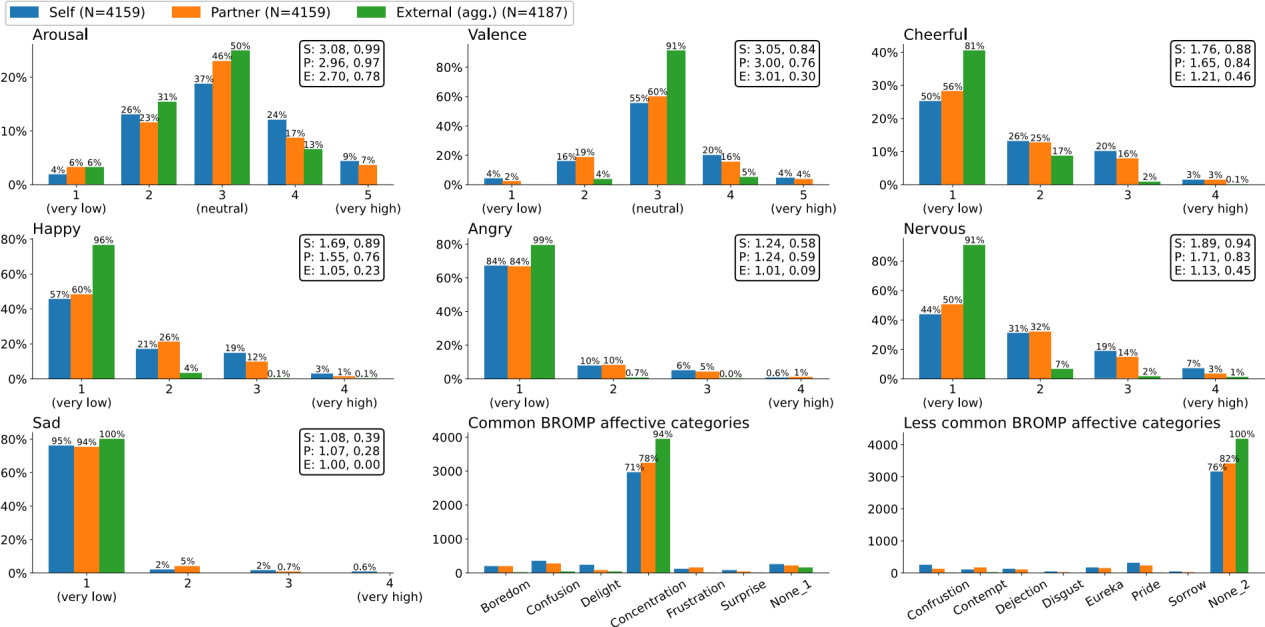
\includegraphics[width=.95\linewidth]{Distributions.frequencies.png}
    \caption[自我(S)、同伴(P)和外部评价者(E)三个角度的情感注释的分布和频率]{自我(S)、同伴(P)和外部评价者(E)三个角度的情感注释的分布和频率,外部注释通过多数投票汇总。每种情绪和情感类别的注释在32个受试者中进行了汇总。部分图表右上角显示了三个角度测量的平均数和标准差。}{\label{fig:Distributions.frequencies}}
\end{figure}
\begin{figure}[htbp]
    \centering
    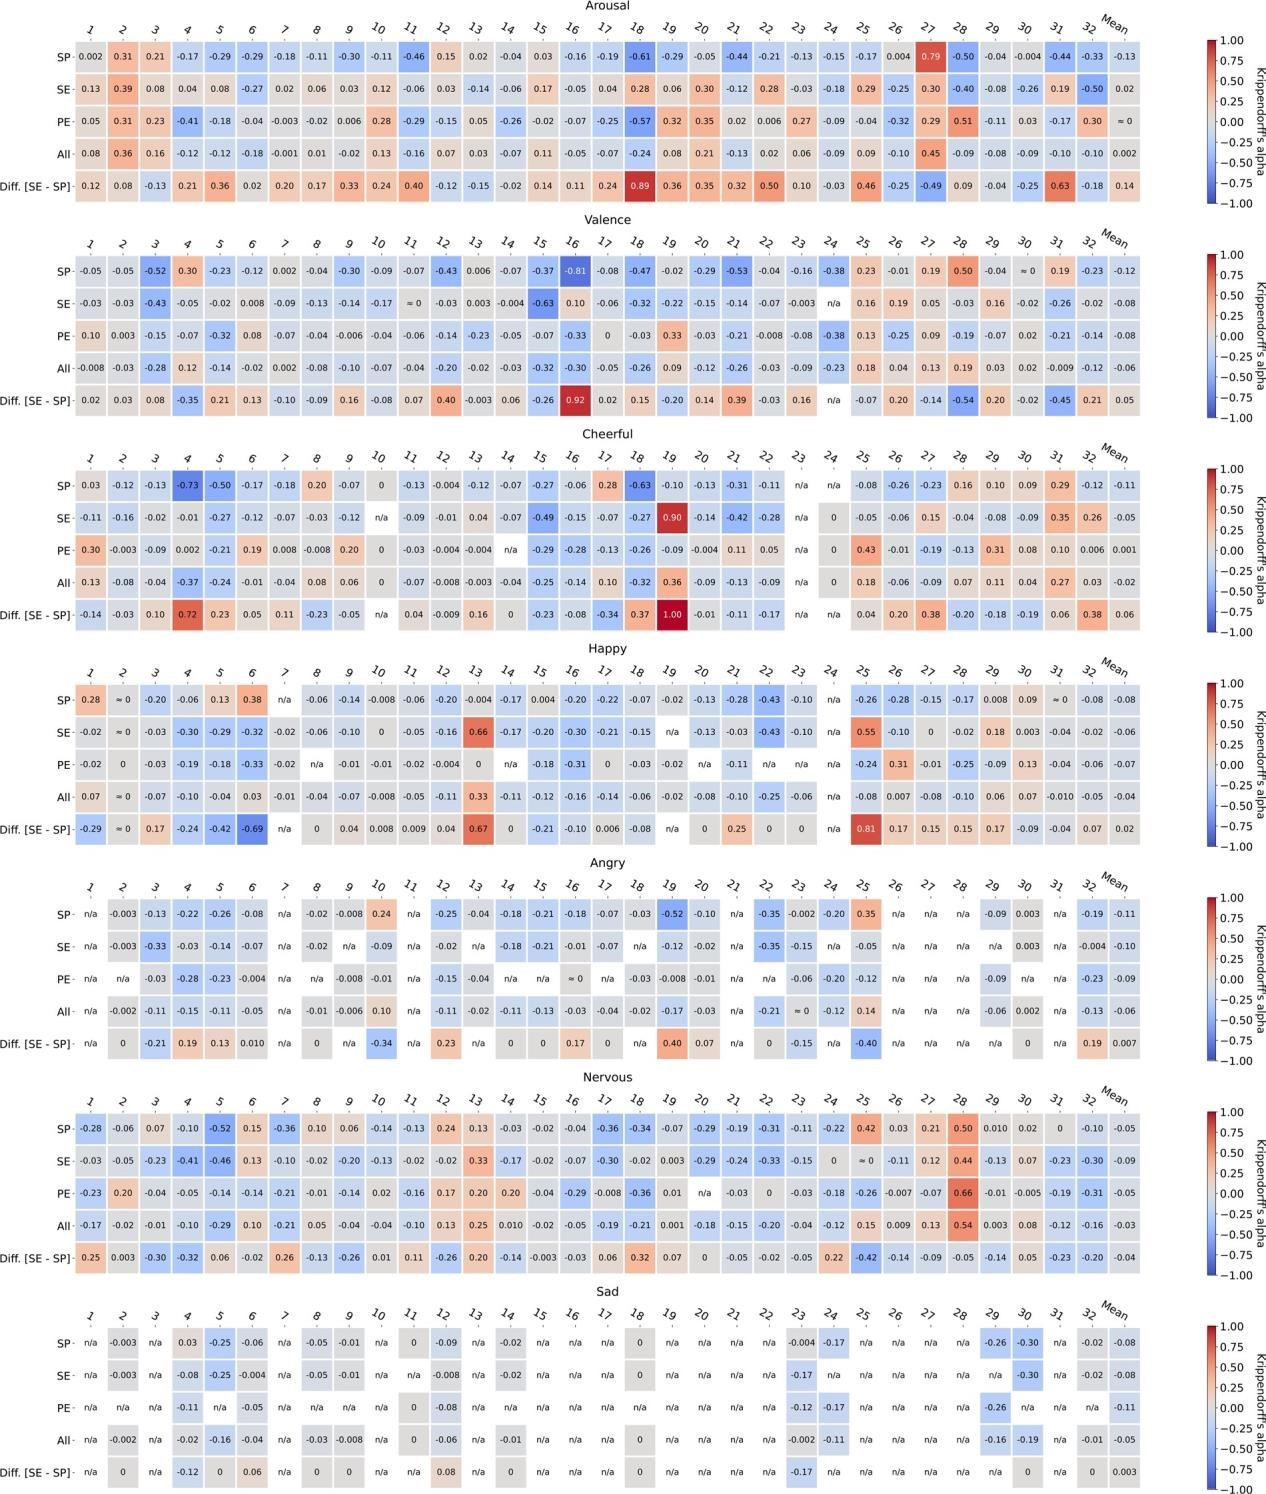
\includegraphics[width=1.0\linewidth]{Heatmaps.jpg}
    \caption[使用Krippendorff's alpha计算的评分员间可信度的热图]{使用Krippendorff's alpha计算的评分员间可信度的热图,外部注释通过多数投票汇总。每个热图的前4行显示四个不同注释角度的α系数:(1) SP为自己对同伴,(2) SE为自己对外部,(3) PE为同伴对外部,(4) 为自己对同伴及外部;最后一行(Diff [SE - SP])显示了自己对外部和自己对同伴之间的差异。各列显示每个参与者的情况。}{\label{fig:Heatmaps}}
\end{figure}

因此,我们对情感注释结果进一步使用模式减法处理,使得α系数能够衡量评分者对情感相对变化的认同程度,而不是他们彼此之间的绝对认同程度。这种调整能够一定程度上减轻从原始注释中获得虚假低α系数值的情况(实现模式减法和绘制热图的代码详见“代码可用性”部分)。

这些固定的α系数通常较低。值得关注的是,在比较自我同伴(SP)注释和自我外部(SE)注释的α系数时,出现了一个比较明显的模式。
如\autoref{fig:Heatmaps}热图中最后一行(Diff. [SE - SP])所示,SE注释和SP注释的IRRs之间的差异往往高于零
(数据来源:22名参与者的唤醒度数据,平均值为0.145,标准差为0.279)。这种模式可能表明,不同角度对情绪的感知可能存在有意义的差异,但其意义的验证还需要进一步的研究。

\subsection{生理信号}
\subsubsection{数据质量}
数据集中生理信号的测量质量已全部检查完成,检查结果作为数据集的一部分包含在data\_quality\_tables.tar.gz打包文件中。
\subsubsection{缺少的数据}
由于数据收集过程中出现设备故障的情况,4名参与者(P2、P3、P6和P7)的E4数据不予使用。
其他生理信号基本没有错误,大部分文件的完整度在95\%以上,但由于设备的固有问题或人为失误,数据部分缺失,具体情况如下:
\begin{itemize}
    \item IBI — P26数据缺失,可能是由于E4内部算法在从BVP推导IBI的过程中,自动舍去了可信度低于设定阈值的数据所致。
    \item EDA — P17和P20数据缺失,可能是由于设备与参与者的皮肤接触不良所致。
    \item NeuroSky(Attention,Meditation)— P1和P20测量结果缺失,P19(32\%)、P22(59\%)和P23(36\%)部分数据丢失,可能是由于设备不完善所致。BrainWave数据未丢失。
    \item Polar HR — 7名参与者(P3、P12、P18、P20、P21、P29和P30)数据丢失,可能是由于数据收集过程中的设备错误所致。
    \item P4(38\%)和P22(38\%)部分数据丢失,可能是由于因接触不良所致。
\end{itemize}

\section{使用说明}
\subsection{潜在应用}
除了之前提到的数据集的预期用途之外,个人生理反应能力的生理标记与积极/消极情绪体验之间的关系,还存在不确定性。我们的数据集可能有助于研究基于生理信号的标记在评估个体使用情绪调节策略方面(如认知评估)的作用。

此外,各种数据挖掘和机器学习的方法可以被应用于建立基于传感器进行生理和行为记录的个人情绪档案模型。这些模型还可以进一步运用到各类实用案例中,为社会创造积极的价值,比如帮助自闭症儿童进行社会交流,帮助盲人阅读面部表情并获得同伴的情绪信息,寻找用户对话的互动时机,帮助社会焦虑症患者克服病情,让机器人更智能地与人互动,以及监测沮丧、情绪饱和等影响驾驶员注意力的迹象,以提高驾驶安全。

\subsection{局限性}
\subsubsection{数据收集装置}
接触型脑电图传感器容易受到噪音的影响(例如,皱眉或眼睛的相关运动可能会造成数据峰值),其他设备也可能受到此类系统误差的影响。
\subsubsection{数据收集的背景}
轮流辩论的背景设置可能导致参与者不断调节甚至压制他们的情绪表达,因为个体往往不会在辩论中不加约束地表露自己的情绪。这就可能导致自我报告和同伴/外部情绪感知之间的一致性降低,进而与自然状态下的互动效果相悖。
\subsubsection{用第二人称镜头进行回溯性情绪注释}
我们使用的回溯性情感判断方法,是让参与者在观看第二人称录像时注释感受到的情绪。这种方法存在一定的缺陷,由于它会涉及到内感受、情绪推理和自我感知之间复杂的相互作用,所以可能会对自我情绪评价产生意想不到的影响。但是我们仍然选择该种注释方法,主要有两个方面的原因:第一个方面的理由在本章节的“情绪注释”部分中已经进行了详细的说明;第二个方面则是考虑到我们的数据集还包括来自辩论同伴和外部评分员对参与者的情绪注释,这不仅弥补了数据集的缺陷,还为研究上述影响开辟了新的视角,同时还能通过比较多角度的情绪感知进行更加全面地研究。
\subsubsection{IRR计算中的模式减法}
模数减法处理后的评分员间可信度值,代表了评分员在相对情绪变化上的一致性,而不是绝对意义上的情绪感知(详见“评分员间可信度”部分)。研究人员在使用数据集之前应关注这一注意事项,确定模数减法处理是否适用于他们的特定用例。
\subsubsection{人口统计资料}
参与者的人口统计资料很可能在数据中引入了偏向。我们所有的参与者和评分员都比较年轻(年龄在19到36岁之间),并受过高等教育,同时大多数为亚洲人。因此,我们的数据可能不能很好地适用于不同种族或年龄更小/大的人群。
\subsubsection{未考虑的变量}
数据收集过程中有很多未考虑的变量,如辩论双方的默契程度、英语口语能力和对辩论主题的熟悉程度等,这些都可能导致情感认知不匹配程度在各个方面上的差异。
\section{代码可用性}
实现离群值检测(Chauvenet标准)、多数投票、模式减法和其他实用功能(热图生成等)的Python代码(3.6.9版本)可以在https://github.com/KaistICLab/K-EmoCon\_SupplementaryCodes找到。Krippendorff软件包(https://github.com/pln-fingudelar/fastkrippendorff)用于计算Krippendorff α系数。

SQL数据库的原始日志级数据通过Python中的SQLAlchemy软件包预处理为CSV文件。因为隐私敏感信息的公开限制,具体代码和原始的日志级数据不予提供。如果数据集用户需要进一步的帮助或有关原始数据及其预处理的信息,欢迎随时与我们联系。
